\fancyfoot[C]{Sandri}
\section{Elektrische Antriebsmaschinen}
Elektrische Maschinen wandeln elektrische Energie in mechanische Energie um, indem sie das Prinzip der Lorenzkraft beziehungsweise Reluktanzkraft anwenden um einen Rotor zu rotieren. Der grunds�tzliche Aufbau eines elektrischen Motors besteht grunds�tzlich aus einem Stator, dem nicht-rotierendem Teil, und einem Rotor, dem sich rotierenden teil. Je nach Typ und Ausf�hrung des Motors sind auf beiden Komponenten Wicklungen beziehungweise Dauermagnete befestigt. Bei einigen Motoren sind auch noch andere Bauteile verbaut.

\subsubsection{Lorentzkraft}
	Die Lorentzkraft wirkt auf bewegliche Lasungstr�ger in einem Magnetfeld. Sie wirkt senkrecht zur Bewegungsrichtung der Ladung und senkrecht zu den Feldlinien des Magnetfelds. Wie sich die Lorentzkraft verh�lt, l�sst sich anhand folgendem Beispiel, einer Leiterschaukel erkl�ren:

	\begin{figure}[H]
			\centering
			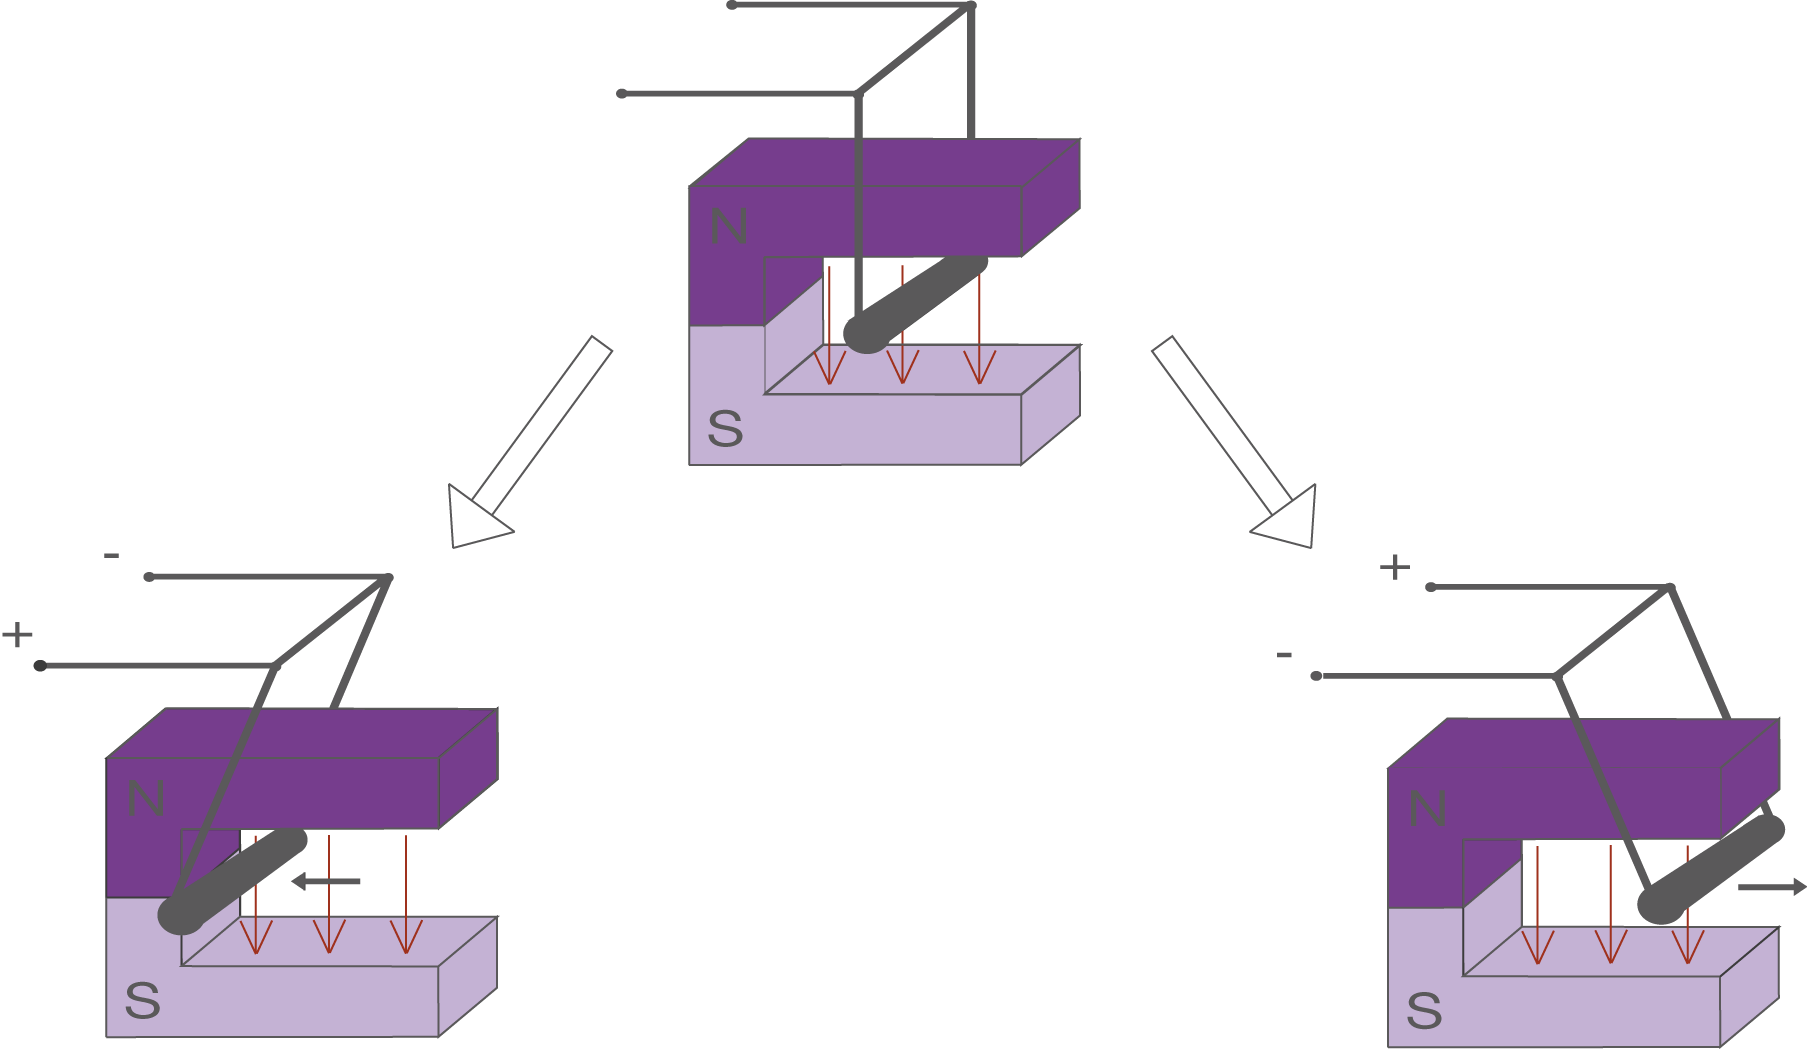
\includegraphics[scale=0.8]{./3_Stand_der_Technik/Abbildungen/Leiterschaukel_1}
			\caption{�nderung der Stromrichtung Lorentzkraft\cite{schullv.de2024}}
	\end{figure}
	
	Die Richtung in welche die Leiterschaukel ausschl�gt, ist zum einen Abh�ngig von der Richtung des Stroms und zum anderen von der Orientierung des Magnetfelds.
	
	\begin{figure}[H]
			\centering
			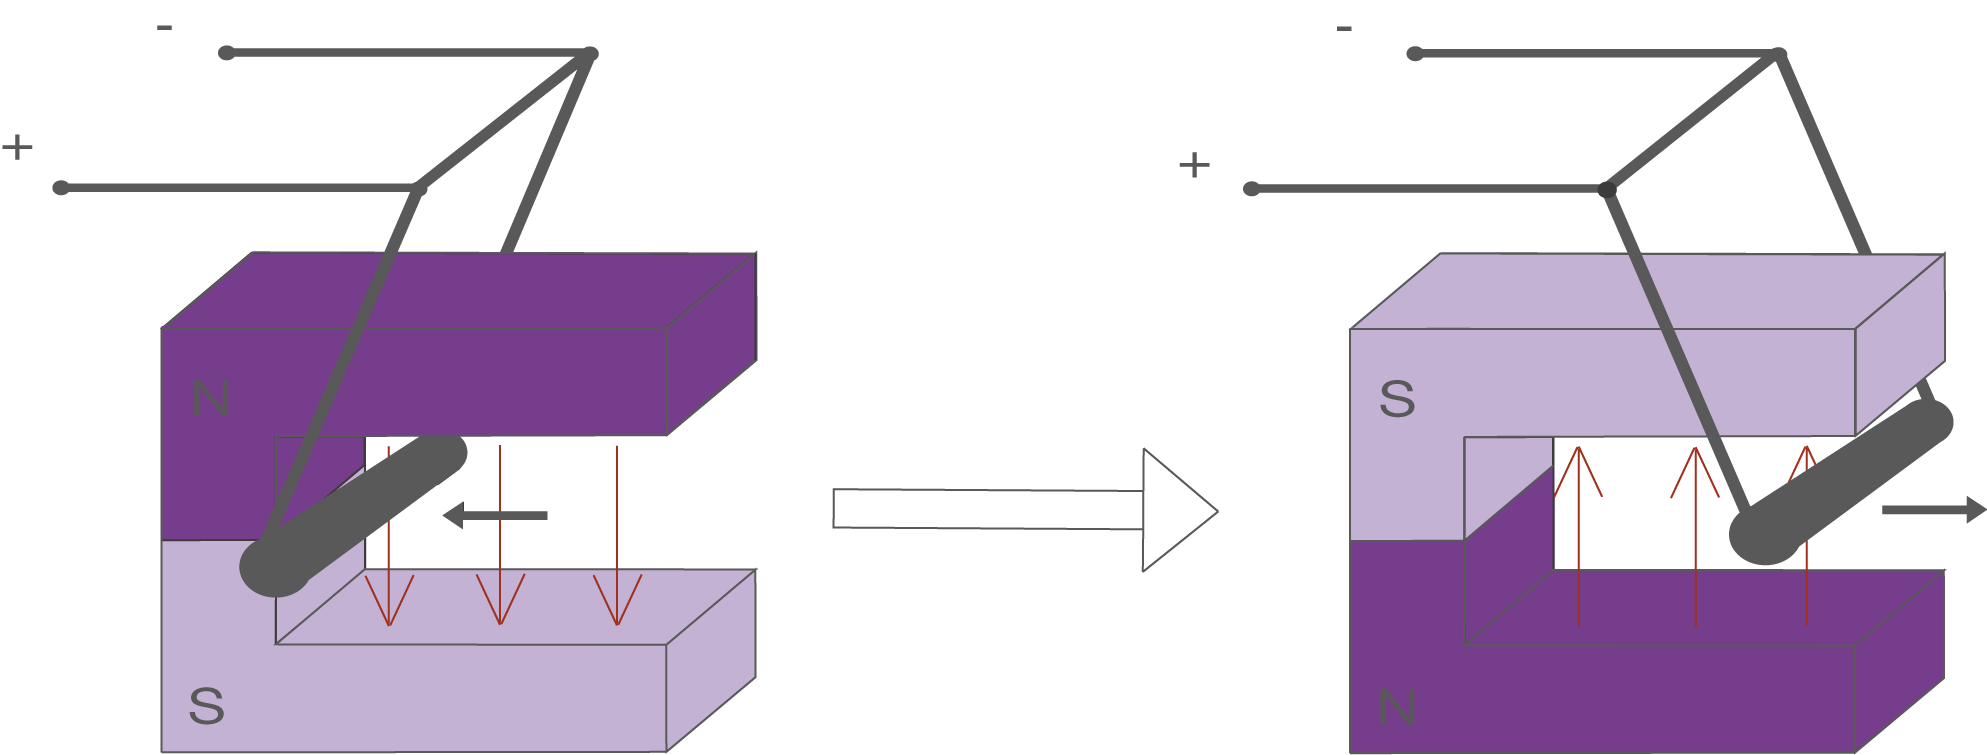
\includegraphics[scale=0.8]{./3_Stand_der_Technik/Abbildungen/Leiterschaukel_2}
			\caption{�nderung des Magnetfelds Lorentzkraft\cite{schullv.de2024}}
	\end{figure}
	
	Die Richtung der Lorentzkraft kann auch durch einen einfachen Versuch, den linke Hand Versuch, ermittelt werden:
	
	\begin{figure}[H]
			\centering
			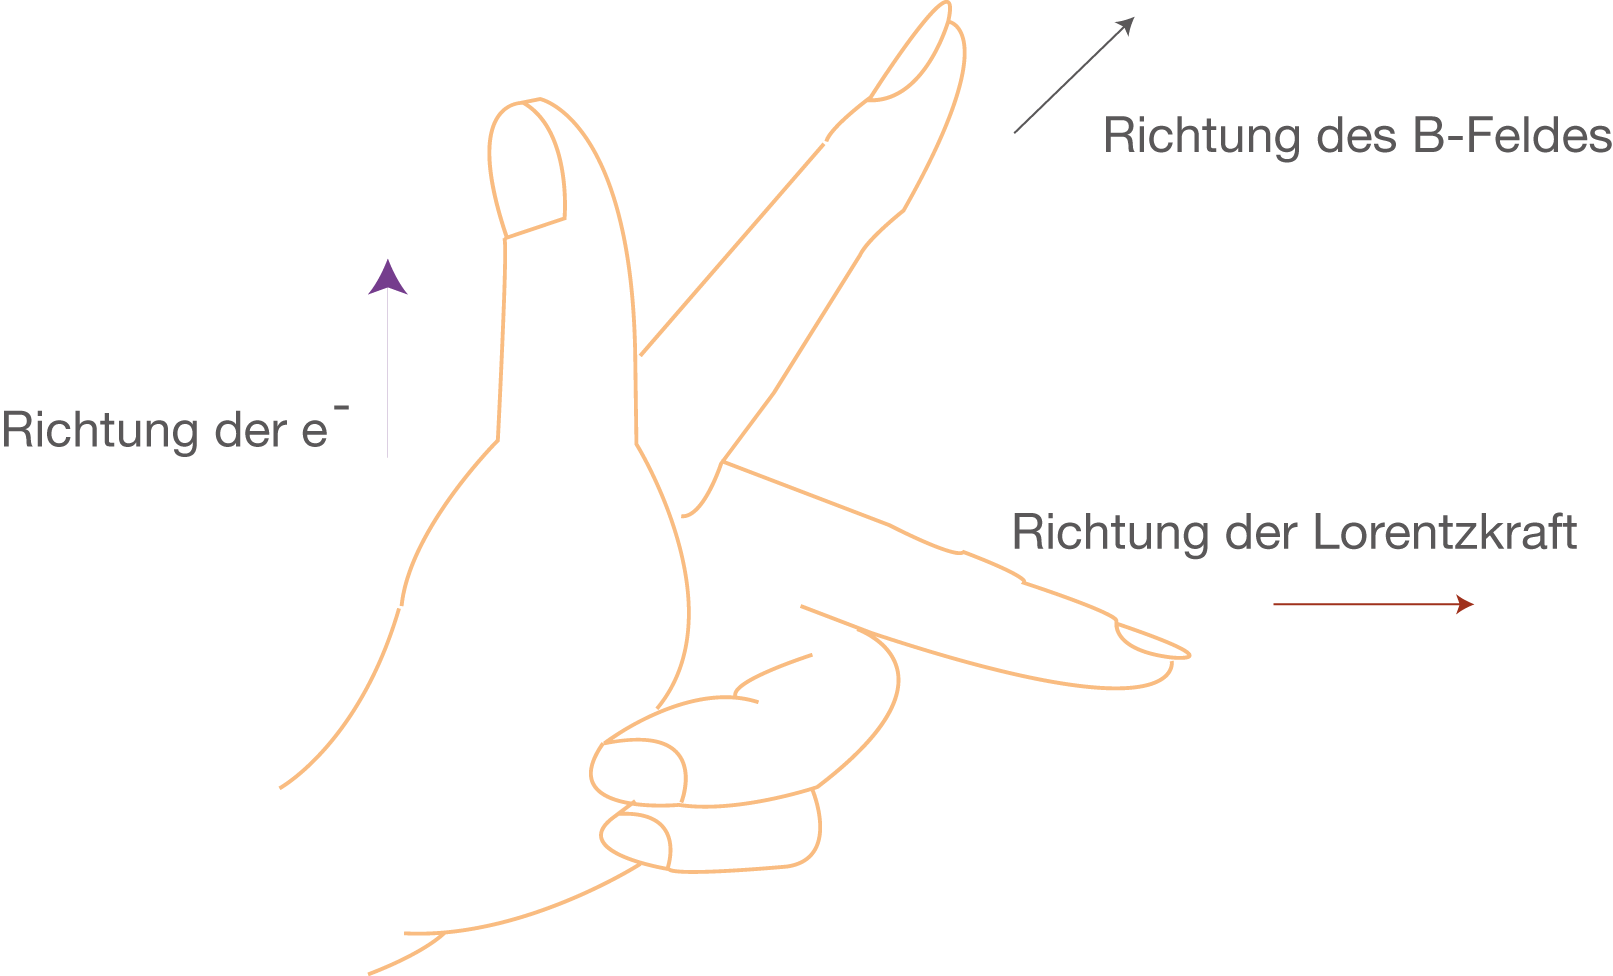
\includegraphics[scale=0.8]{./3_Stand_der_Technik/Abbildungen/Lorentzkraft_1}
			\caption{Die linke Hand Regel\cite{schullv.de2024}}
	\end{figure}

	Mathematisch kann die Richtung der Lorentzkraft mihilfe des Kreuzprodukts aus der Magnetfeldrichtung und der Bewegungsrichtung der Elektronen errechnet werden:
	
	\begin{equation}
		\vec{F_{L}} = q * (\vec{v_{e}} \times \vec{B})
	\end{equation}
	
	Der Betrag kann wiefolgt errechnet werden:
	
	\begin{equation}
		F_{L} = q*v*B*\sin{\alpha}
	\end{equation}
	
	Wobei der Winkel $\alpha$ den Winkel zwischen der Bewegungsrichtung der Elektronen und der Bewegungsrichtung des Magnetfelds entspricht. Auch kann man anhand dieser Formel erkennen, dass die Lorentzkraft null wird, wenn die Bewegungsrichtung der Elektronen und die des Magnetfelds parallel verl�uft.\cite{schullv.de2024}
	
	Die meisten elektrischen Maschinen funktionieren grunds�tzlich aufgrund der Lorentzraft, es gibt jedoch vereinzelt Maschinen, die nur aufgrund der Reluktanzkraft funktionieren.

\subsubsection{Reluktanzkraft}

	Die Reluktanzkraft (auch Maxwellsche Kraft genannt) entsteht durch �nderung des magnetischen Widerstands. Sie wirkt immer so, dass sich der magnetische Widerstand verringert und die Induktivit�t steigt. Diese Kraft kann durch Ver�nderung des Luftspalts im magnetischen Kreis erzeugt werden.\cite{biancahoegel.de/2021}
	
	\subsection{Asynchronmaschine}
	Die Asynchronmaschine ist die einfachste Form einer elektrischen Maschine. Sie wird angetrieben durch ein Drehfeld, welches durch eine mehrstr�ngige Wicklung im Stator erzeugt wird. Der gro�e Vorteil des Asynchronmaschine ist ihre einfache Bauform und Funktionsweise. Auch bedarf sie nur geringer Wartung. Der gro�e Nachteil hingegen ist jedoch seine startk an die Frequenz der Eingangsspannung gebundene Drehzahl. Im gebr�uchlichen 50-Hz-Betrieb sind nur Drehzahlen von 3000U/min, 1500U/min, 1000U/min, abh�ngig von der Anzahl der Polpaare.
	
	\begin{equation}
		n \thickapprox f / p
	\end{equation}
	
	n $\cdots$ Motordrehzahl \newline
	f $\cdots$ Frequenz vom Netz	\newline
	p $\cdots$ Anzahl der Polpaare \newline
	
	Es gibt haupts�chlich zwei Typen der Asynchronmaschine, den K�figl�ufer und den Schleifringl�ufer. Der K�figl�ufer verwendet also Rotor eines Stahlk�fig, der Schleifringl�ufer hat Schleifringe, �ber die Wicklungen im Rotor bestromt werden.
	
	\begin{figure}[H]
			\centering
			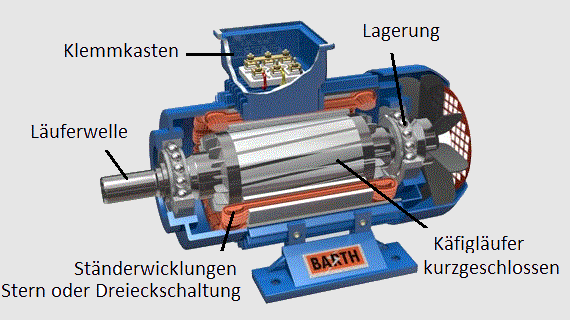
\includegraphics[scale=0.6]{./3_Stand_der_Technik/Abbildungen/Asynchronmaschine_2}
			\caption{Aufbau K�figl�ufer\cite{kfzaufgaben.de2024}}
	\end{figure}
	
	\begin{figure}[H]
			\centering
			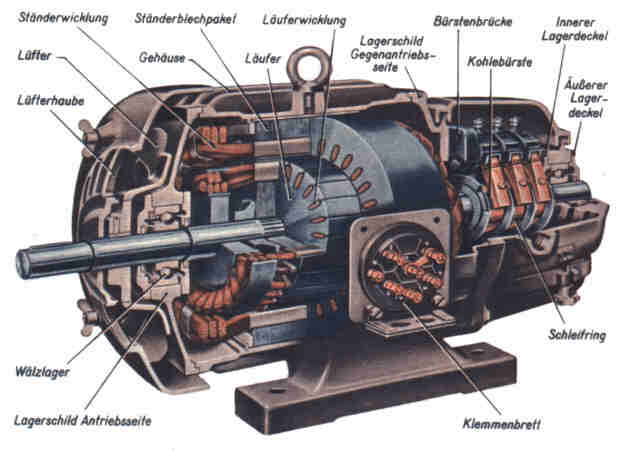
\includegraphics[scale=2]{./3_Stand_der_Technik/Abbildungen/Asynchronmaschine_3}
			\caption{Aufbau Schleifringl�ufer\cite{wupperindustrie.de2024}}
	\end{figure}

	Betrieben wird die Asynchronmaschine indem sie an das 3-phasige 50Hz-Netz angeschlossen wird. Sie dreht sich dadurch fast synchron mit der Netzfrequenz. Asynchronmaschinen laufen ihrem Feld jedoch immer etwas hinterher, diese Eigenschaft nennt man Schlupf. Das Drehmoment- und Drehzahlverhalten kann sehr gut mittels eines Kreisdiagramms dargestellt werden.\cite{Fischer2017}
	
	\begin{figure}[H]
			\centering
			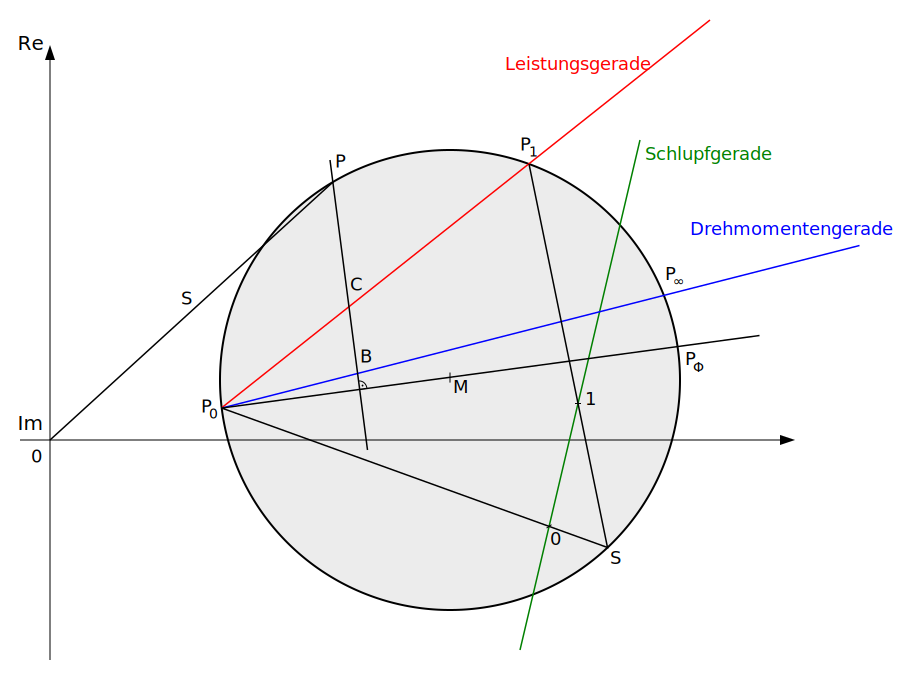
\includegraphics[scale=0.4]{./3_Stand_der_Technik/Abbildungen/Kreisdiagramm_1}
			\caption{Kreisdiagram eines Asynchronmotors\cite{Wikipedia2024}}
	\end{figure}
	
	
	
	\subsection{Gleichstrommaschine}
	
	\subsection{Synchronmaschine}
	
	\subsection{Permanenterregte Synchronmaschine}
	
	\subsection{Positionsmessung}
	
	\subsection{Trapezf�rmige Regelung}
	
	\subsection{Feldorientierte Regelung}